\documentclass[a4paper,titlepage,final, twoside]{report}

% Page size
\usepackage{a4wide}

% Fonts and Language Support
\usepackage[english]{babel}
\usepackage[utf8]{inputenc}
\usepackage[T1]{fontenc}
\usepackage{mathtools}
%\usepackage{newtxtext,newtxmath}
\usepackage{setspace}
\usepackage{fancyhdr}
%\usepackage{fixme}
\usepackage{graphicx}
%\usepackage{caption}
%\usepackage{subcaption}
%\usepackage{float}
\usepackage{listings}
\usepackage{underscore} % så behøver vi ikke escape underscores i tekst, fx til links
\usepackage{lastpage}
%\usepackage{pdfpages}
%\usepackage{longtable}
\usepackage{xfrac}
%\usepackage{sidecap}
\usepackage{caption}
\usepackage{subcaption}
\usepackage{enumitem}
\usepackage{xcolor}
\usepackage[framemethod=tikz]{mdframed}
\usepackage[a4paper,width=150mm,top=25mm,bottom=25mm,bindingoffset=6mm]{geometry}
\usepackage[]{algorithm2e}
\usepackage[authoryear]{natbib}

% Macros
\newcommand{\HRule}{\rule{\linewidth}{0.5mm}}
\newcommand{\degree}{\ensuremath{^\circ}}
\newcommand{\code}[1]{\texttt{#1}}
\renewcommand{\arraystretch}{1.5}

%mdframed settings
\mdfdefinestyle{mystyle}{%
linecolor=blue!40!black,outerlinewidth=1pt,%
frametitlerule=true,frametitlefont=\sffamily\bfseries\color{white},%
frametitlerulewidth=1pt,frametitlerulecolor=blue!40!black,%
frametitlebackgroundcolor=blue!40!black,
backgroundcolor=blue!5,
innertopmargin=\topskip,
roundcorner=5pt
}
\newmdenv[style=mystyle]{exa}
\newenvironment{example}[1]
  {\begin{exa}[frametitle=#1]}
  {\end{exa}}

%listing settings
\lstset{frame=tbrl, aboveskip=1mm, belowskip=1mm, showstringspaces=false, columns=flexible, basicstyle={\scriptsize\ttfamily}, breaklines=true, tabsize=3}


%marks
\let\Chaptermark\chaptermark
\def\chaptermark#1{\def\Chaptername{#1}\Chaptermark{#1}}
\let\Sectionmark\sectionmark
\def\sectionmark#1{\def\Sectionname{#1}\Sectionmark{#1}}
\let\Subsectionmark\subsectionmark
\def\subsectionmark#1{\def\Subsectionname{#1}\Subsectionmark{#1}}
\let\Subsubsectionmark\subsubsectionmark
\def\subsubsectionmark#1{\def\Subsubsectionname{#1}\Subsubsectionmark{#1}}

% Style setup
%\setlength{\headheight}{15pt}
\pagestyle{fancy}
\fancyhead{}
\fancyhead[RO,LE]{\rightmark}
\fancyhead[RE,LO]{\leftmark}
\fancyfoot{}
\fancyfoot[LE,RO]{\thepage}





% Header and footer
%\lhead{Truco: A South American Card Game (Group 10, ITU10)}
%\rfoot{\fancyplain{}{Page \thepage\ of \pageref{LastPage}}}
%\cfoot{}

% Frontpage
\begin{document}

% diverse
%\parindent=0pt % Ingen indrykning
%\parskip=8pt plus 2pt minus 4pt

\setcounter{page}{0}

% Abstract
\begin{spacing}{1.5}
\begin{abstract}
	Lorem ipsum dolor sit amet, consectetur adipisicing elit, sed do eiusmod tempor incididunt ut labore et dolore magna aliqua. Ut enim ad minim veniam, quis nostrud exercitation ullamco laboris nisi ut aliquip ex ea commodo consequat. Duis aute irure dolor in reprehenderit in voluptate velit esse cillum dolore eu fugiat nulla pariatur. Excepteur sint occaecat cupidatat non proident, sunt in culpa qui officia deserunt mollit anim id est laborum.
\end{abstract}
\end{spacing}

% TOC
\tableofcontents
\newpage


%------------------------------------------------------------------------------------------------------------------------------%
%------------------------------------------------------------------------------------------------------------------------------%
%------------------------------------------------------------------------------------------------------------------------------%
\chapter{Introduction}


%------------------------------------------------------------------------------------------------------------------------------%
%------------------------------------------------------------------------------------------------------------------------------%
%------------------------------------------------------------------------------------------------------------------------------%
\chapter{Background}
The idea of generating complete games through algorithms is not itself new. The problem in full generality is quite large, so usually a subset of the general problem is tackled. Videogames may be comprised of a large number of tangible and intangible components, including rules, graphical assets, genre conventions, cultural context, controllers, character design, story and dialog, screen-based information displays, and so on~\citet{cook2014angelina,liapis2014creativity,nelson2007automated}.

In this paper we look specifically at generating game rules; and more specifically the rules of arcade-style games based on graphical movement and local interaction between game elements, represented in the game description language VGDL. The two main approaches that have been explored in generating game rules are reasoning through constraint solving~\citet{smith2010variations} or search through evolutionary computation or similar forms of stochastic optimisation~\citet{togelius2008experiment,browne2008automated,font2013towards}. In either case, rule generation can be seen as a particular kind of procedural content generation~\citet{pcgbook:ch6}.

It is clear that generating a set of rules that makes for an interesting and fun game is a hard task. The arguably most successful attempt so far, Browne's Ludi system, managed to produce a new board game of sufficient quality to be sold as a boxed product~\citet{browne2008automated}. However, it succeeded partly due to restricting its generation domain to only the rules of a rather tightly constrained space of board games. A key stumbling block for search-based approaches to game generation is the fitness/evaluation function. This function takes a complete game as input and outputs an estimate of its quality. Ludi uses a mixture of several measures based on automatic playthrough of games, including balance, drawishness and outcome uncertainy. These measures are well-chosen for two-player board games, but might not transfer that well to video games or single-player games, which have in a separate analysis been deemed to be good targets for game generation~\citet{togelius2014characteristics}. Other researchers have attempted evaluation functions based on the learnability of the game by an algorithm~\citet{togelius2008experiment} or an earlier and more primitive version of the characteristic that is explored in this paper, performance profile of a set of algorithms~\citet{font2013towards}.


\section{Content generation}
Procedural content generation is a topic that is being increasingly researched and implemented in games of various types and genres (source). PCG can help game designers in creating game elements like levels/maps, environments, weapons or AI's.

\citet{hendrikx2013procedural} suggests a six-layered taxonomy to describe PCG at different stages of games, while performing a survey of different ways in which PCG have been implemented.

\subsection{Game-level generation}
Almost all video games are highly dependent on designed level or map (or levels/map) in which the game play takes place. Levels are often responsible for creating increasingly challenging situations, and thereby entertaining game play. Super Mario would be way less interesting if enemies and platforms were spread randomly across each level, which would almost certainly result in the game being ether too easy or too difficult.

In recent years, game developers have begun using automatic generation of game-levels, to decrease the human work-load while still creating interesting content for games. Using PCG for creating "dungeon"-type maps have long been a successful endeavor for certain type of games as seen in \textit{Rogue} \citeyearpar{game:rogue}, the \textit{Diablo}-series, and in newer times \textit{Minecraft} \citeyearpar{game:minecraft} and \textit{Spelunky} \citeyearpar{game:spelunky}. PCG were additionally successfully implemented in strategy games like "Civilization II", "Command \& Conquer: Tiberian Sun" and "XCom: UFO Defense", but otherwise automatically generating levels have not been hugely successful in other game genres.

Several scientific projects have focused on the topic as well with an array of different approaches, some requiring player-input, or simply a helper for human level-designer. In addition to the other game genres mentioned above, a lot of work has been done in generating levels for puzzle games (ie. Sokoban and Cut The Rope).
Most of the work is focused on generating levels for single game, where some attempt to create general level generation procedures.


\subsection{Other uses of PCG}
Other games have been published applying PCG in different ways. In \textit{Borderlands 2} \citeyearpar{game:borderlands} the player have access to an extreme amount of different weapons, designed by automatic generation.


\subsection{Advantages and disadvantages using PCG}

Having a procedure for generating content in games has a number of advantages:

\begin{itemize}
  \item Content generation allows games to potentially have an endless amount of possibilities, often resulting in higher re-play value than linear games. 
  \item PCG can help game designers generate game levels, often simply by letting the designer explore possible layouts, add decorations or finishing up human-designed levels.
\end{itemize}

PCG also has some problems for generating content for levels:

\begin{itemize}
  \item Generated content can have a feeling of being unauthentic and/or too random. For instance, the positions of decorations in a level (barrels, paintings etc.) can be important for humans, while they are not for computers.
  \item In games where the player follows a story it can be difficult to automatically generate levels, that follow what the game designer intend to happen%.
\end{itemize}




\section{Game generation}
Generating complete games is a topic that has not been researched very much. Additionally very little success has been achieved, with the only the exception being the game generation project Ludi.

A typical approach for generating complete games is searching in a space of possible games. This basically requires two things: That the ratio of enjoyable games in the set is not too low - otherwise those games might never be found. To increase this ratio a game description language (GDL) is often used (searching through all possible Java or C programs would lead to an enormous amount invalid games).
Also, to search through a set of games it is necessary to be able to calculate a fitness value for each game, valuing how enjoyable the game is.

\subsection{Game description languages}
Regardless of which approach to game generation is chosen, one needs a way to represent the games that are being created.\footnote{See \citet{pcgbook:ch6} for a discussion of game-rule representation choices.} For a sufficiently general description of games, it stands to reason that the games are represented in a reasonably generic language, where every syntactically valid game description can be loaded into a specialised game engine and executed. 

\subsubsection*{Stanford GDL}
There have been several attempts to design such GDLs. One of the more well-known is the Stanford GDL, which is used for the General Game Playing Competition~\citet{genesereth2005general}. That language is tailored to describing board games and similar discrete, turn-based games; it is also arguably too verbose and low-level to support search-based game generation. 

\subsubsection*{PuzzleScript}
Another attempt at an VGDL is called PuzzleScript, created by game designer Stephen Lavelle. The language (as its name suggest) is focused on turn-based puzzle games, but the engine allows for simple forms of animation and movement. The language is relatively high level compared to Stanford GDL, but does not support that large set of video games.


\subsubsection*{VGDL}
The various game generation attempts discussed above feature their own GDLs of different levels of sophistication; however, there has not until recently been a GDL for suitably for a larger space of video game types- and genres.
The Video Game Description Language (VGDL) is a GDL designed to express 2D arcade-style video games of the type common on hardware such as the Atari 2600 and Commodore 64. It can express a large variety of games in which the player controls a single moving avatar (player character) and where the rules primarily define what happens when objects interact with each other in a two-dimensional space. VGDL was designed by a set of researchers~\citet{levine2013general,ebner2013towards} (and implemented by Schaul ~\citet{schaul2013video}) in order to support both general video game playing and video game generation.
In contrast to other GDLs, the language has an internal set of classes, properties and types that each object can defined by, which the authors suggest the user to extend.

Objects have physical properties (i.e. position, direction) which can be altered either by the properties defined, or by interactions defined between specific objects. 
The games take place on a specified level constructed from game-tiles, however objects are able to move slowly between game-tiles.

A VGDL description has four parts: 

\begin{description}
\item [SpriteSet] Defines which sprites can appear in the game. Each sprite must be designated by a class, in which a set of predefined actions exists. Also a set of parameters can be fed to each sprite, configuring for instance the speed or how often the sprite takes an action, and the parameters used for the different sprite-classes -- for instance, for the  class \textbf{Flicker} (a simple extension to the base sprite, the sprite is destroyed after a speecifed amount of time) the lifetime can be adjusted.
Sprites can additionally be designed in a tree structure, where multiple sprites have the same parent sprite, making more possibility for the interactions and terminations described below. 
\item [InteractionSet] Each line defines what happens when a set of two sprites collide with each other (located on the same game-tile). Each interaction is represented by a class defining the action to take (i.e. push back, or kill sprite), and a set of parameters specific to each interaction-class, as well as the score achieved for letting the interaction happen.
\item [TerminationSet]
\item [LevelMapping]
\end{description}
%the SpriteSet, which defines the ontology of the game -- which sprites exist and what can they do; the LevelMapping, which maps from level description to game state; the InteractionSet, which defines what happens when sprites overlap, and the TerminationSet which defines how the game can be won or last.


\begin{figure}[!ht]
\centering
\begin{lstlisting}
BasicGame
	SpriteSet
		city  > Immovable color=GREEN img=city
		explosion > Flicker limit=5 img=explosion
		movable >
			avatar  > ShootAvatar stype=explosion
			incoming >
				incoming_slow  > Chaser stype=city color=ORANGE speed=0.1
				incoming_fast  > Chaser stype=city color=YELLOW speed=0.3

	LevelMapping
		c > city
		m > incoming_slow
		f > incoming_fast
		
	InteractionSet
		movable wall  > stepBack
		incoming city > killSprite
		city incoming > killSprite scoreChange=-1
		incoming explosion > killSprite scoreChange=2

	TerminationSet
		SpriteCounter stype=city   win=False
		SpriteCounter stype=incoming win=True
\end{lstlisting}
\caption{Example of VGDL description - a simple implementation of the game Missile Command}
\label{fig:vgdl}
\end{figure}



\subsection{The GVG-AI Framework}

The GVG-AI framework is a testbed for testing general gameplaying controllers against games specified using VGDL. Controllers are called once at the beginning of each game for setup, and then once per clock tick to select an action. Controllers do not have access to the VGDL descriptions of the games. They receive only the game's current state, passed as a parameter when the controller is asked for a move. However these states can be forward-simulated to future states. Thus the game rules are not directly available, but a simulatable model of the game can be used.

The framework additionally contains 20 hand-designed games, which mostly consist of interpretations of classic video games. Figure \ref{fig:vgdl} shows the VGDL description of the game \emph{Missile Command}.
Most of the games are inspired by classic arcade- and Atari games (e.g. Boulderdash, Frogger, Missile Command and Pacman), while some are original creations by the General Video-Game AI Competition's organizers. 
The games can in general be described (except for \emph{Sokoban}) as action arcade games, in that the player controls a single avatar which must be moved quickly around in a 2D-setting to win, or to get a high score (the player is able to increment a score  counter in all of the games).



Below is a short summary of each of games, describing the winning conditions, and how the player can increase his/her score:
\begin{description}
\item [Aliens] VGDL interpretation of the classic arcade game \emph{Space Invaders}. A large amount of aliens are spawned from the top of the screen. The player wins by shooting all the approaching aliens.\\
\textbf{Goal} Destroy all the incoming aliens, without being hit by them or their projectiles.\\
\textbf{Scoring} Destroy all the incoming aliens, without being hit by them or their projectiles.
\item [Boulderdash] VGDL interpretation of \emph{Boulder Dash}. The avatar has to dig through a cave to collect diamonds while avoiding being smashed by falling rocks or killed by enemies. 
\item [Butterflies] The avatar has to capture all butterflies before all the cocoons are opened. Cocoons open when a butterfly touches them.
\item [Chase] About chasing and killing fleeing goats. However, if a fleeing goat encounters the corpse of another, it get angry and start chasing the player instead.
\item [Digdug] VGDL interpretation of \emph{Dig Dug}. Avatar collects gold coins and gems, digs his way through a cave and avoid or shoot boulders at enemies.
\item [Eggomania] VGDL interpretation of \emph{Eggomania}. Avatar moves from left to right collecting eggs that fall from a chicken at the top of the screen, in order to use these eggs to shoot at the chicken, killing it.
\item [Firecaster] Goal is to reach the exit by burning wood that is on the way. Ammunition is required to set things on fire.
\item [Firestorms] Player must avoid flames from hell gates until he finds the exit of a maze.
\item [Frogs] VGDL interpretation of \emph{Frogger}. Player is a frog that has to cross a road and a river, without getting killed.
\item [Infection] Objective is to infect all healthy animals. The player gets infected by touching a bug. Medics can cure infected animals.
\item [Missile Command] VGDL interpretation of the classic arcade game \emph{Missile Command}. Player has to destroy falling missiles, before they reach their destinations. If the player can save at least one city, he wins.
\item [Overload] Player must get to the level after collecting coins, but cannot collect too many coins, as he will be too heavy to traverse the exit.
\item [Pacman] A VGDL interpretation of \emph{Pac-Man}. Goal is to clear a maze full with power pills and pellets, and avoid or destroy ghosts.
\item [Portals] Objective is to get to a certain point using portals to go from one place to another, while at the same time avoiding lasers.
\item [Seaquest] VGDL interpretation of \emph{Seaquest}. Avatar is a submarine that rescue divers and avoids sea animals that can kill it. The goal is simply to a high score.
\item [Survive Zombies] Player has to flee zombies until time runs out, and can collect honey to kill the zombies.
\item [Whackamole] VGDL implementation of the classic arcade game \emph{Whac-a-Mole}. Must collect moles that appear from holes, and avoid a cat that mimics the moles.
\item [Zelda] VGDL interpretation of \emph{Legend of Zelda}. Objective is to find a key in a maze and leave the level. Player also has a sword to defend himself against enemies.
\item [Camelrace] Player needs to get to endpoint to win.
\item [Sokoban] The objective is to move the boxes to holes, until all boxes disappear or the time runs out.
\end{description}

%------------------------------------------------------------------------------------------------------------------------------%

\subsection{Game genres describable in VGDL}
The VGDL implementation of the GVG-AI competetion is essentially (without great extension) only able to describe certain action-arcade games, and puzzle games.
For instance, the lack of possibility to traverse different levels make \textbf{Adventure} games impossible to make, and the restriction of only being able move a single character with the keyboard (the avatar) makes great restriction in creating \textbf{Strategy} games.

In this project we will focus on the two main type of games describable in VGDL: Action-arcade games and turn-based puzzle games. We make the simple distinction that arcade games contain elements (sprites) that move by themselves, whereas interactions only occur as a result of the avatar moving in puzzle games.
This puts the game \emph{Portals} in the arcade genre, even though it contains puzzle elements.

To increase the size of the set of designed games, and to allow for more precise analysis we created a series of fourteen new game descriptions in VGDL. However the most important reason for creating new descriptions, was to introduce a series of \emph{puzzle games} to be analyzed.
All of these games are interpretations of classic (pre-1990) games, and the levels 
Below is short description of each of these games:

\begin{description}
\item [Bait] VGDL interpretation of the classic arcade game \emph{Space Invaders}. A large amount of aliens are spawned from the top of the screen. The player wins by shooting all the approaching aliens.\\
\textbf{Goal} Destroy all the incoming aliens, without being hit by them or their projectiles.\\
\textbf{Scoring} Destroy all the incoming aliens, without being hit by them or their projectiles.
\item [The Citadel] VGDL interpretation of \emph{Boulder Dash}. The avatar has to dig through a cave to collect diamonds while avoiding being smashed by falling rocks or killed by enemies. 
\item [Bombuzal] The avatar has to capture all butterflies before all the cocoons are opened. Cocoons open when a butterfly touches them.
\item [Chip's Challenge] About chasing and killing fleeing goats. However, if a fleeing goat encounters the corpse of another, it get angry and start chasing the player instead.
\item [Bolo Adventures] VGDL interpretation of \emph{Dig Dug}. Avatar collects gold coins and gems, digs his way through a cave and avoid or shoot boulders at enemies.
\item [(Real) Sokoban] VGDL interpretation of \emph{Eggomania}. Avatar moves from left to right collecting eggs that fall from a chicken at the top of the screen, in order to use these eggs to shoot at the chicken, killing it.
\item [Brainman] Goal is to reach the exit by burning wood that is on the way. Ammunition is required to set things on fire.
\item [Modality] Player must avoid flames from hell gates until he finds the exit of a maze.
\item [Painter] VGDL interpretation of \emph{Frogger}. Player is a frog that has to cross a road and a river, without getting killed.
\item [Zen Puzzle] Objective is to infect all healthy animals. The player gets infected by touching a bug. Medics can cure infected animals.
\end{description}


Four new arcade/action games were introduced as well, to increase the number of games of designed games in analyses. 
\begin{description}
\item [Crackpots] VGDL implementation of the classic arcade game \emph{Whac-a-Mole}. Must collect moles that appear from holes, and avoid a cat that mimics the moles.
\item [Solar Fox] VGDL interpretation of \emph{Legend of Zelda}. Objective is to find a key in a maze and leave the level. Player also has a sword to defend himself against enemies.
\item [Astroblast] Player needs to get to endpoint to win.
\item [Centipede] The objective is to move the boxes to holes, until all boxes disappear or the time runs out.
\end{description}

%------------------------------------------------------------------------------------------------------------------------------%



%------------------------------------------------------------------------------------------------------------------------------%
\section{Puzzle games}
A large amount of games contain puzzle-elements, but only a few has puzzles as the main game-play.



%------------------------------------------------------------------------------------------------------------------------------%
%------------------------------------------------------------------------------------------------------------------------------%
%------------------------------------------------------------------------------------------------------------------------------%
\chapter{Research Objectives}
The main objectives of this study was to create a generator being able to create simple games and levels, enjoyable for human players.
The focus of the study was to create fitness functions able to differentiate between games (and levels) of different quality, to be able to create interesting content. Making the generator able to create a large amount of games, and then select the ones with the highest quality.

\section{General Evaluation - Arcade-/Action Games}
The first goal was to use the results of a series of general game-playing (knowledge free) algorithms to value a given game.

\section{Breadth First Search - Puzzle Games}
The second goal was to 

\section{Assumptions}
We assume that the games metioned are of high quality (i.e. highly enjoyable for human players). This is not always clear when playing the games in their form, since they need crucial element to keep a game fun: Audio, graphic effects, control-scheme fiiting to the games.
We reason this because they are clones of existing games.


%------------------------------------------------------------------------------------------------------------------------------%
%------------------------------------------------------------------------------------------------------------------------------%
%------------------------------------------------------------------------------------------------------------------------------%

\chapter{Methodology}
This section describes the experimental- setup, and methodology used in achieving the research objectives.

\section{Arcade-/action games}
\label{sec:actiongames}

\subsection{Example games: Arcade-/action}
Two of the 20 games from the GVG-AI framework were deemed too monotonous after initial tests. 
In these two games the controllers all had similar scores for each run - or with only one controller being able to increase its score.
The remaining 18 hand-designed VGDL game descriptions were chosen to be used as a baseline for testing and game generation. 

%Most of the games are inspired by classic arcade- and Atari games (e.g. Boulderdash, Frogger, Missile Command and Pacman), while some are original creations by the General Video-Game AI Competition's organizers. 

%The games can in general be described as action arcade games, in that the player controls a single avatar which must be moved quickly around in a 2D-setting to win, or to get a high score (the player is able to increment a score  counter in all of the games).


\subsection{Mutation of example games}
\label{method:mutation}
A mutation process was repeatedly applied for each of the 18 example games mentioned in section \ref{method:examples}. 
The process consisted of changing the set of interaction rules (i.e. lines from the InteactionSet) defined in each game description.
For each mutation, each interaction rule had a $25\%$ chance of being mutated, but with a requirement that at least one rule were changed. 
Mutation occured by changing the objects in that interaction rule, the function on collision between said objects, and/or the function's parameters.

Several contrains were used during each mutation to avoid games with non-valid descriptions (which can cause crashes in the GVG-AI framework).
Additionally, several constraints were used for the different function parameters, as to only allow "realistic" values. 
The range of these constraints were extrapolated (and slightly extended) from the example games. 
For instance, the parameter \emph{limit} used by certain rules was limitied to values between 0 and 10, as the same is true for the rules of the example games. 
This process was applied 20 times for each example game description, resulting in 360 generated game descriptions.

When testing the mutated games the same level descriptions as for their original counterparts were used (those mentioned in section \ref{method:examples}).




\subsection{Random game generation}
\label{method:random}

A set of 400 random VGDL game descriptions were generated by constructing the textual lines for different parts of a VGDL description: Generating an array of sprites (for the SpriteSet), interaction-rules (InteractionSet), termination-rules (TerminationSet) and level mappings (LevelMapping).


%\begin{figure}[ht]
%	\centering
%	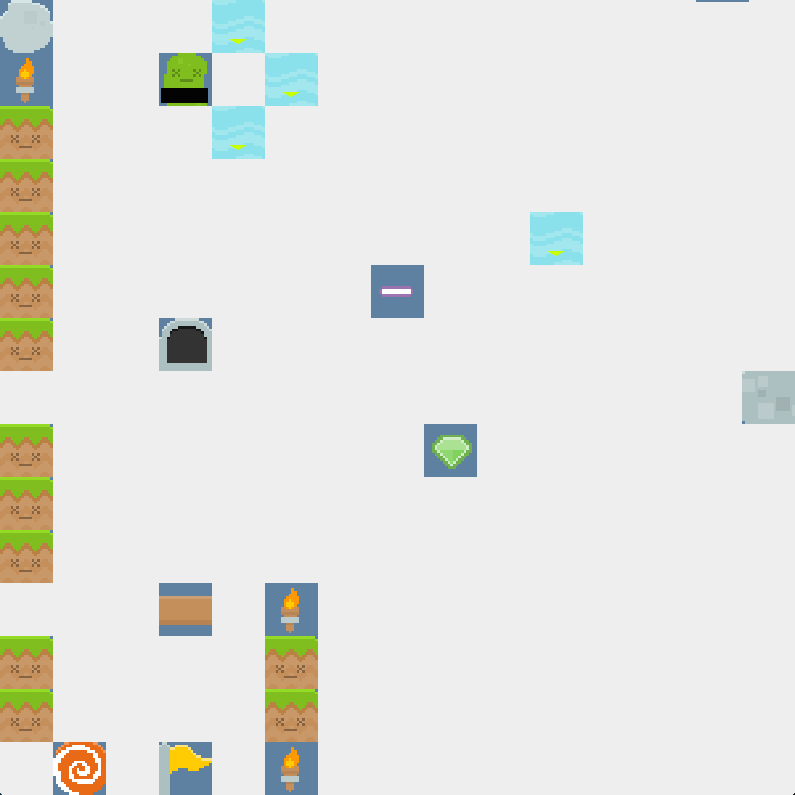
\includegraphics[width=0.45\textwidth]{gengame.png}
%	\caption{Visual representation of one of the 400 randomly generated VGDL games}
%\end{figure}

Before generating descriptions, we used similar constraints to those mentioned in section~\ref{method:mutation}, partly to avoid generating descriptions with invalid elements, and partly to increase the proportion of interesting outcomes. 
The number of sprites, interaction- and termination-rules were randomly chosen, limited to 25, 25, and 2, respectively. Furthermore, a simple level description (only containing one of each sprite) was generated for each of the generated game descriptions for test purposes. 


%------------------------------------------------------------------------------------------------------------------------------%

\section{Turn-based puzzle games}

\subsubsection*{Definition of games}
The games described in this section are games where the puzzles are the only game-play. There is no fast movement, or quick reaction time required to win. Additionally, because the games are described using the GVG-AI framework, the games focus around a player avatar which can only move up, down, left or right (also, in the games described below, all movement are from one game-tile to another).

\subsection{Games} 
Description of the puzzle games used in tests.

\subsection{Level generation} 
A setup for creating levels for a given game were constructed using an evolutionary algorithm. The level generator described in section \ref{sec:actiongames} was used to generate simple levels for games.  In addition two extra options were added: Wall-sprites and ground-sprites. This reduces a lot of troubles since the avatar would otherwise be able to escape the level in a lot of the games. Ground-sprites signify which sprite should appear on empty locations.

\subsubsection*{Mutation} 



\subsubsection*{Crossover} 
Two different levels were constructed into a new, by going over each tile on the level and with 50\% chance take the sprite residing in the two different original levels.


The setup was as follows:
\\

\begin{algorithm}[H]
 %\KwData{this text}
 %\KwResult{how to write algorithm with \LaTeX2e }
% initialization\;
 \While{not at end of this document}{
  read current\;
  \eIf{understand}{
   go to next section\;
   current section becomes this one\;
   }{
   go back to the beginning of current section\;
  }
 }
 \caption{How to write algorithms}
\end{algorithm}



\subsection{Level generation for generated games} 


\begin{example}{The Title}
Put here cool text like what is going on in the wauw
\end{example}
This is subsubsection with title ``\Subsectionname''.

%------------------------------------------------------------------------------------------------------------------------------%
%------------------------------------------------------------------------------------------------------------------------------%
%------------------------------------------------------------------------------------------------------------------------------%

\chapter{Results}

\section{Action-arcade games: Setup}
Om det vi lavede i paperet (+ mine egne spil PL0X!)

\subsection{Generated games}
About how the games were generated.

\subsection{Mutated games}
About mutated games

\subsection{Outcome}
The conclusion of the above tests is that the the result distribution of controllers can be used to score a game, with a high probability.


\section{Action-arcade games: Fitness functions}
From the above tests we can see that it is interesting to write a fitness function for controllers results, to be able to find out if new generated games are of a high quality.


\subsection{Action-arcade games: Generated levels}
Results of what happens when generating levels for the example games.





% Body
%\begin{spacing}{1.5}
%\input{./introduction.tex}
%\input{./process-description.tex}
%\input{./structural-overview.tex}
%\input{./behavioral-overview.tex}
%\input{./points-of-interest.tex}
%\end{spacing}

%Bibliography
%\newpage
%\addcontentsline{toc}{section}{References}
%\begin{thebibliography}{9}
%	\bibitem{hacking_roomba}
%	  Kurt, T. E.,
%	  \emph{Hacking Roomba},
%	  Wiley Publishing.
%	  2007.
%\end{thebibliography}

\bibliography{bigliography}
\bibliographystyle{plainnat}

% Appendices
\newpage
\appendix

\end{document}
